%%%%%%%%%%%%%%%%%%%%%%% file template.tex %%%%%%%%%%%%%%%%%%%%%%%%%
%
% This is a template file for Web of Conferences Journal
%
% Copy it to a new file with a new name and use it as the basis
% for your article
%
%%%%%%%%%%%%%%%%%%%%%%%%%% EDP Science %%%%%%%%%%%%%%%%%%%%%%%%%%%%
%
%%%\documentclass[option]{webofc}
%%% "twocolumn" for typesetting an article in two columns format (default one column)
%
\documentclass{webofc}
\usepackage[varg]{txfonts}   % Web of Conferences font
%
% Put here some packages required or/and some personnal commands
%
%
\begin{document}
%
\title{Insert your title here}
%
% subtitle is optionnal
%
%%%\subtitle{Do you have a subtitle?\\ If so, write it here}

\author{\firstname{Brad} \lastname{Rawlins}\inst{1,3}\fnsep\thanks{\email{rwlbra001@myuct.ac.za}} \and
        \firstname{Ryno} \lastname{Laubscher}\inst{2}\fnsep\thanks{\email{ryno.laubscher@uct.ac.za}} \and
        \firstname{Pieter} \lastname{Rousseau}\inst{3}\fnsep\thanks{\email{pieter.rousseau@uct.ac.za}}
        % etc.
}

\institute{University of Cape Town 
\and
           the second here 
\and
           Last address
          }

\abstract{%
  The use of a thermal non-equilibrium Eulerian-Eulerian model for the simulation of a 620 MWe power
boiler is proposed for capturing the combustion and radiative heat transfer found in the pulverized fuel systems. The models eliminates the use of a Lagrangian reference frame in tracking solid fuel particles thereby reducing the computational expense and time. The model solves the scalar transport for the particle mass, energy and radiation interactions between the pseudo-particle and continuous phases.\\
The model is validated against both numerical and applicable site data measurements. It is shown that the model is able to adequately resolve the furnace and super-heater wall heat fluxes. Additionally the models ability to resolve the flow field, combustion dynamics and wall fluxes is demonstrated for 80 %
and 60 % operational load characteristics.
}
%
\maketitle
%
\section{Introduction}
\label{intro}
Your text comes here. The paper should not exceed 12 pages (including the list of references). Separate text sections with
fgfjdfjsbv

\section{Section title}
\label{sec-1}
For bibliography use \cite{RefJ}
\subsection{Subsection title}
\label{sec-2}
Don't forget to give each section, subsection, subsubsection, and
paragraph a unique label (see Sect.~\ref{sec-1}).

For figures use syntax of figure~\ref{fig-1}
\begin{figure}[h]
% Use the relevant command for your figure-insertion program
% to insert the figure file.
\centering
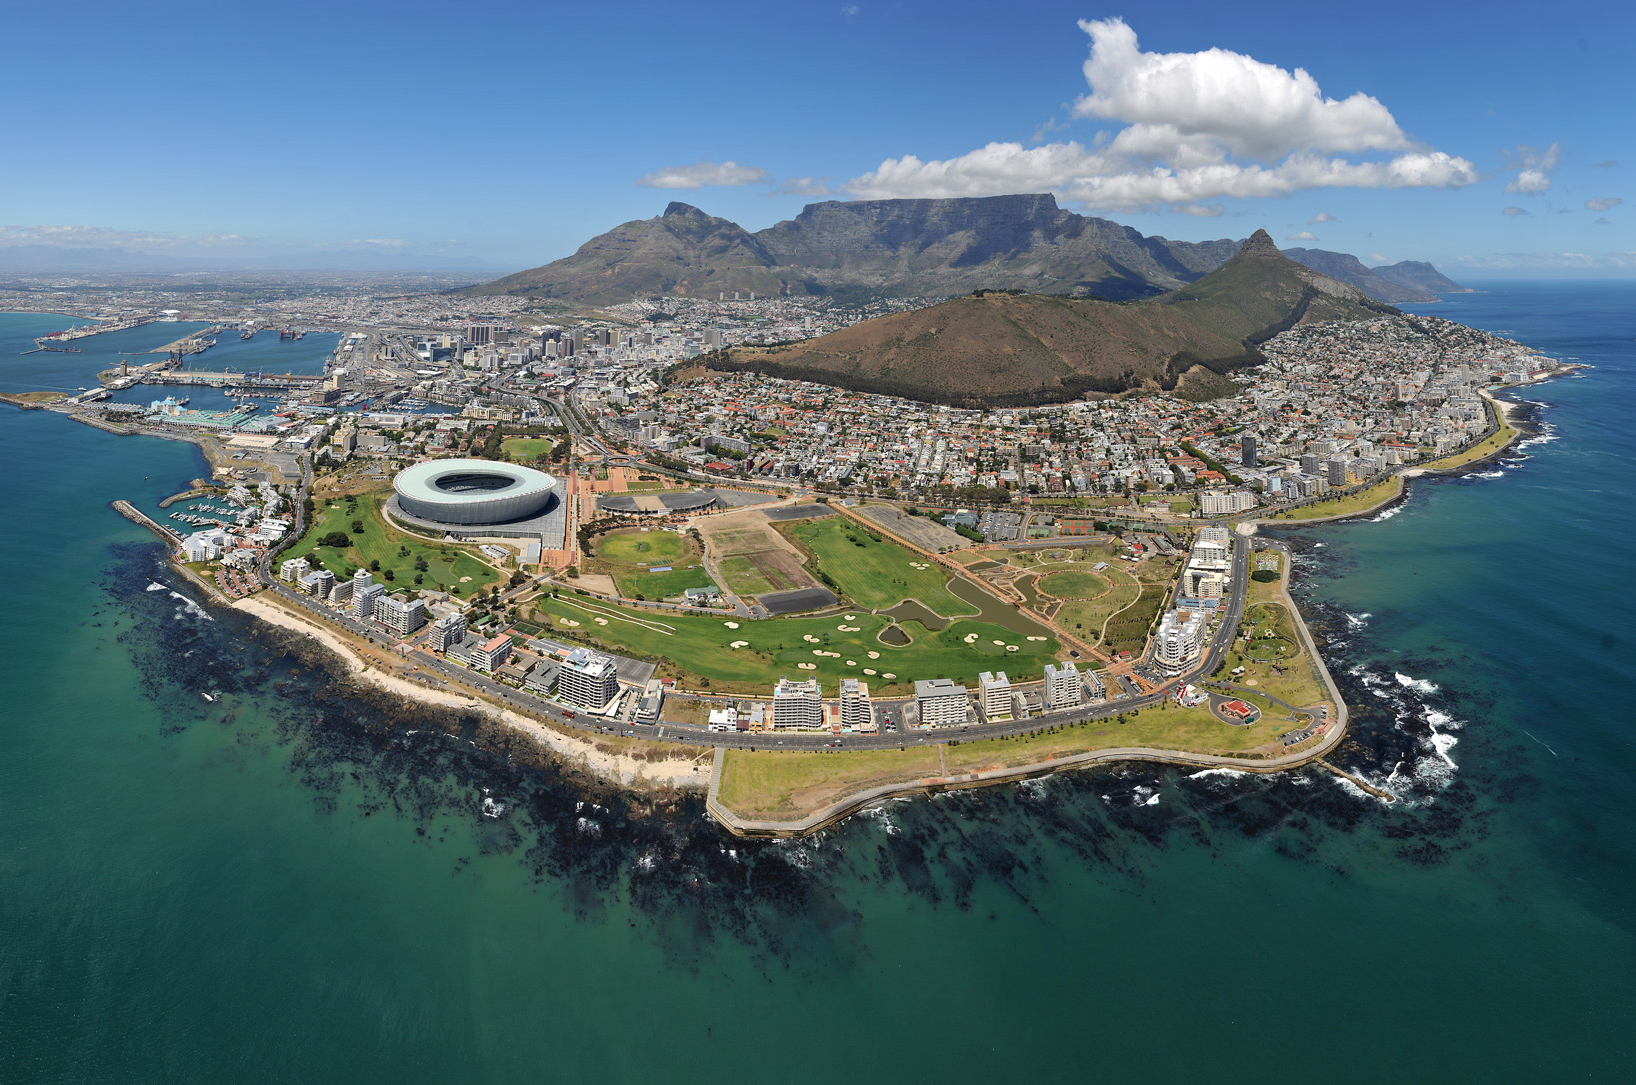
\includegraphics[width=10cm,clip]{cape_town.png}
\caption{Please write your figure caption here}
\label{fig-1}       % Give a unique label
\end{figure}

For tables use syntax in table~\ref{tab-1}.
\begin{table}
\centering
\caption{Please write your table caption here}
\label{tab-1}       % Give a unique label
% For LaTeX tables you can use
\begin{tabular}{lll}
\hline
first & second & third  \\\hline
number & number & number \\
number & number & number \\\hline
\end{tabular}
% Or use
\vspace*{5cm}  % with the correct table height
\end{table}
%
% BibTeX or Biber users please use (the style is already called in the class, ensure that the "woc.bst" style is in your local directory)
% \bibliography{name or your bibliography database}
%
% Non-BibTeX users please use
%
\begin{thebibliography}{}
%
% and use \bibitem to create references.
%
\bibitem{RefJ}
% Format for Journal Reference
Journal Author, Journal \textbf{Volume}, page numbers (year)
% Format for books
\bibitem{RefB}
Book Author, \textit{Book title} (Publisher, place, year) page numbers
% etc
\end{thebibliography}

\end{document}

% end of file template.tex

<div id='footer'><table width='100%'><tr><td class='right'><a href='http://fusioninventory.org/'><span class='copyright'>FusionInventory 9.1+1.0 | copyleft <img src='/glpi/plugins/fusioninventory/pics/copyleft.png'/>  2010-2016 by FusionInventory Team</span></a></td></tr></table></div>